%% The basic ESPResSo tutorial
%%
% Writer's guide lines:
% - provide background information and references
% - do not get lost in details but maintain a nice readability
% - describe every line of the script, that contains an ESPResSo
%   command (in future tutorial, only describe new ones)
%
%%%%%%%%%%%%%%%%%%%%%%%%%%%%%%%%%%%%%%%%%%%%%%%%%%%%%%%%%%%%%%%%%
%%%%%%%%%%%%%%%%%%%%%%%%%%%%%%%%%%%%%%%%%%%%%%%%%%%%%%%%%%%%%%%%%
% From the brainstorming:
%
% Preknowledge:
%
% Basic MD(simple integrator,langevin thermostat, ---basic tcl
% basic potentials, basis tutorial 1
%
% Basis Tutorial: written in Latex
%
% <<every line of script code should be explained>>
%
% 1) tcl basic setting up a system
% MD, soft sphere and Lennard-Jones Fluid (argon system),
% Units
%
% online visualization (pdb output)
% rdf, pressure,energy,
%
% online analysis function
% savin, readin writeout, offline analysis, statistics
%
% Structure:
% Part1:
% 1) Prerequisits (what you should know beforehand: basic tcl knowledge,
% Here you can find more info: Allen, Tildesley: Frenkel smit,
% Rappaport, tcl tutorial,
%
% 2) Physics of the systems (argon, soft sphere system)
%
% 3) Algorithms (verlocity verlet, Langevin, Potentials, LJ)
% 3b) about units
%
% Part2
% 1) simulation script in all detail, line by line
% Initialize
% Visualize
% Simulate (with online analysis, saves for later off-line analysis,
% (Savelize (save our lives ))
%
% 2) a new script for later
% analysis, and other helper ideas
%
% Things to remember and take care of:
% Use the same names for variables
%
% ====================================================================
% General Tutorial: (the next tutorials: pe_solution, cell model of one
% charged colloid, LB, ferrofluid)
%

% basiert auf KOMA-Script scrbook-Klasse
\documentclass[11pt,a4paper,% BCOR8mm,
	       %twoside, onecolumn, openright, cleardoubleempty, %
	       %parindent,
headnosepline, footnosepline, notitlepage, %
	       %onelinecaption,
bigheadings, % bibtotoc, %tocindent, listsindent, %
	       %chapterprefix, noappendixprefix,
	       %tablecaptionbelow,
	       %pointlessnumbers, % macht Probleme (Anhang ohne Punkt, aber sonst Kapitel mit Punkt
	       % abstractoff, fleqn, leqno,
	       % openbib, origlongtable,
final]{scrartcl}

% Satzspiegel

% wenn keine KOMA-Klasse verwendet wird, kann so der Satzspiegel
% berechnet werden
%\usepackage[DIV15,BCOR12mm,pagesize]{typearea}

% Hier knnen Seitenhoehe und -breite individuell angepasst werden
%\areaset[BCOR]{Breite}{Hohe}
% oder
%\usepackage[a4paper,body={15.6cm,23cm},left=3cm]{geometry}

% ============================================================================

%% Grafikpakete
% Fr einfache Einbingung von Grafiken
\usepackage{graphicx}%
\usepackage{framed, color}

% Wenn man direkt mit dem pdflatex eine PDF-Datei erzeugt, sollten diese beiden
% Pakete eingebunden werden (Hyperlinks, bessere Bildschirmschriftarten usw.)
\usepackage{color}
\definecolor{mylinkcolor}{rgb}{0.5812,0.0665,0.0659} % IndianRed
\definecolor{mycitecolor}{rgb}{0.075,0.31,0.0431} % MossGreen
\definecolor{myurlcolor}{rgb}{0.0118,0.098,0.7412} % DarkBlue
\usepackage[pdftex,bookmarks]{hyperref}

% Druckversion
% f�r reine pdf-Dateien noch Option colorlinks hinzufgen, um Links farbig zumachen
% \usepackage[pdftex,bookmarks,bookmarksopen,citecolor={mycitecolor},%
%  linkcolor={mylinkcolor},urlcolor={myurlcolor},breaklinks=true,%
%  hypertexnames=false,hyperindex=true,encap,colorlinks]{hyperref} %

%  	\hypersetup{
%     pdftitle = {},
%     pdfauthor = {Kai Grass},
%     pdfsubject = {},
%     pdfkeywords = {},
%     pdfcreator = {},%
%     pdfproducer = {},
% 	}%

\usepackage{ae,aecompl}

% ============================================================================

%% Sprachliche Pakete
\usepackage[english]{babel}
% Neue Deutsche Rechtschreibung
%\usepackage[ngerman]{babel}
%\usepackage{ngerman}

% Paket zur einfacheren Eingabe deutscher Umlaute
%\usepackage[applemac]{inputenc} %Mac
\usepackage[latin1]{inputenc}   %UNIX/LINUX
% \usepackage[ansinew]{inputenc}  % Windows
%\usepackage[T1]{fontenc}

% ============================================================================

% Literaturverzeichnis
\usepackage[square,numbers,sort&compress]{natbib}
%\usepackage{bibmods}
%\bibpunct{(}{)}{,}{a}{}{,}
%\bibpunct{(}{)}{,}{a}{,}{;}
\setlength{\bibsep}{1ex}

% ============================================================================

% Stichwortverzeichnis
% \usepackage{makeidx}
% \makeindex

% ============================================================================

% Deutsche Zahlenkonvention (1 (Komma) 0 statt 1 (Punkt) 0)
% \usepackage{ziffer}

%% Schriftarten
\usepackage{times} % times is used to avoid bitmap fonts in PDF

%% Mathematische Packages
% Dieses Pakete definiert viele ntzliche mathematische Befehele und
% Die Option "intlimits" bewirkt, dass beim Integral die Grenzenangaben oben
% und unten erscheinen und nicht seitlich.
\usepackage[intlimits]{amsmath}
\usepackage{amsfonts}
\usepackage{amsthm}
\usepackage{mathrsfs}
\usepackage{stmaryrd}


% Diese Schriftarten ermglichen schne Mengensymbole fr natrliche Zahlen, usw.
% siehe Definition von \N, \Z usw. Dies ist Geschmackssache.
%\usepackage{bbm}
%\usepackage{dsfont}

% Subfigures
\usepackage{subfigure}

% Needed for Tabular-Umgebung
\usepackage{array}

% werden (sog. Schusterjungen und Hurenkinder vermeiden)
%\clubpenalty = 10000
%\widowpenalty = 10000

\sloppy

% Ein Paket um "kommutative Diagramme" zu erstellen. Fuer einfhrende Beispiele
% siehe xymanual.ps und xyreference.ps
%\usepackage[all]{xy}

%%%%%%%%%%%%%%%%%%% Shortcuts %%%%%%%%%%%%%%%%%%%%%%%%%%%%%%%%%%%%%%%%%%%%
%\newcommand{\N}{\mathbbm{N}}	% Natuerliche Zahlen
%\newcommand{\Z}{\mathbbm{Z}}	% Ganze Zahlen
%\newcommand{\Q}{\mathbbm{Q}}	% Rationale Zahlen
%\newcommand{\R}{\mathbbm{R}}	% Reelle Zahlen
%\newcommand{\C}{\mathbbm{C}}	% Komplexe Zahlen
%\newcommand{\one}{\mathbbm{1}}	% Einheits Eins
%
%\newcommand{\toinf}{\to\infty}				% --> oo
%\newcommand{\tozero}{\to 0}				% --> 0
%\newcommand{\ontop}[2]{\genfrac{}{}{0pt}{}{#1}{#2}}	% Aufeinander
%\newcommand{\abs}[1]{\left|#1\right|}
%\newcommand{\argmax}{\mathop{\rm arg\,max}}

% Ein Befehl, um Abbildungen einfach einheitlich zu gestalten
% Bsp: \abb{f}{\R}{\R}{x}{x^2}

%\newcommand{\abb}[5]{%
%\setlength{\arraycolsep}{0.4ex}%
%\begin{array}{rcccc}%
%#1 &:\,& #2 & \,\,\longrightarrow\,\, & #3 \\[0.5ex]%
%     & & #4 & \longmapsto & #5%
%\end{array}%
%}

%%%%%%%%%%%%%%%%%%% Theorem definitions %%%%%%%%%%%%%%%%%%%%%%%%%%%%%%%%%%
%\theoremstyle{plain}
%\newtheorem{theorem}{Theorem}[chapter]
%\newtheorem{proposition}[theorem]{Proposition}
%\newtheorem{lemma}[theorem]{Lemma}
%\newtheorem{satz}[theorem]{Satz}
%\newtheorem{korollar}[theorem]{Korollar}
%
%\theoremstyle{definition}
%\newtheorem{definition}{Definition}[chapter]
%\newtheorem{beispiel}[theorem]{Beispiel}
%\newtheorem{bemerkung}[theorem]{Bemerkung}
%
%%%%%%%%%%%%%%%%%%%%%%%%%%%%%%%%%%%%%%%%%%%%%%%%%%%%%%%%%%%%%%%%%%%%%%%%%%

% ============================================================================
% \renewcommand*{\partpagestyle}{empty}
% \renewcommand*{\partformat}{\partname~\thepart:}
%\usepackage{fancyhdr}
%%\pagestyle{headings}
%\pagestyle{fancyplain}
%%\addtolength{\headwidth}{\marginparsep}
%%\addtolength{\headwidth}{\marginparwidth}
%\renewcommand{\chaptermark}[1]{\markboth{#1}{}}
%\renewcommand{\sectionmark}[1]{\markright{\thesection\ #1}}
%%\lhead[\fancyplain{}{\bfseries\thepage}]{\fancyplain{}{\bfseries\rightmark}}
%\lhead[\fancyplain{}{\thepage}]{\fancyplain{}{\rightmark}}
%%\rhead[\fancyplain{}{\bfseries\leftmark}]{\fancyplain{}{\bfseries\thepage}}
%\rhead[\fancyplain{}{\leftmark}]{\fancyplain{}{\thepage}}
%%\chead{}
%%\rhead{\thepage}
%%\lfoot{Schnellste Pfade in geometrischen Netzwerken}
%\cfoot{}
%%\rfoot{}
%%\setlength{\headrulewidth}{0.4pt}
%%\setlength{\footrulewidth}{0.4pt}

%\usepackage[automark]{scrpage2}
%\pagestyle{scrheadings}
%\automark[section){chapter}
%\lehead[scrplain-links-gerade]{scrheadings-links-gerade}
%\cehead[scrplain-mittig-gerade]{scrheadings-mittig-gerade}
%\rehead[scrplain-rechts-gerade]{scrheadings-rechts-gerade}
%\lefoot[scrplain-links-gerade]{scrheadings-links-gerade}
%\cefoot[scrplain-mittig-gerade]{scrheadings-mittig-gerade}
%\refoot[scrplain-rechts-gerade]{scrheadings-rechts-gerade}
%\lohead[scrplain-links-ungerade]{scrheadings-links-ungerade}
%\cohead[scrplain-mittig-ungerade]{scrheadings-mittig-ungerade}
%\rohead[scrplain-rechts-ungerade]{scrheadings-rechts-ungerade}
%\lofoot[scrplain-links-ungerade]{scrheadings-links-ungerade}
%\cofoot[scrplain-mittig-ungerade]{scrheadings-mittig-ungerade}
%\rofoot[scrplain-rechts-ungerade]{scrheadings-rechts-ungerade}
%\ihead[scrplain-innen]{scrheadings-innen}
%\chead[scrplain-zentriert]{scrheadings-zentriert}
%\ifoot[scrplain-innen]{scrheadings-innen}
%\cfoot[scrplain-zentriert]{scrheadings-zentriert}
% Markierungen: \leftmark, \rightmark, \pagemark \headmark
% \manualmark \automark

% ============================================================================

%%%%%%%%%%%%%%%%%%%%%%%%%%%%%%%%%%%%%%%%%%%%%%%%%%%%%%%%%%%%%%%%%%%%%%%%%%
\setcounter{secnumdepth}{2}
\setcounter{tocdepth}{1}
%%%%%%%%%%%%%%%%%%%%%%%%%%%%%%%%%%%%%%%%%%%%%%%%%%%%%%%%%%%%%%%%%%%%%%%%%%

%% Schriftsatz in KOMA
%\setkomafont{Element}{Befehle}
%\addtokomafont{Element}{Befehle}
%\usekomafont{Element}

%\includeonly{kapitel/sinterkeramiken, kapitel/statisch, kapitel/dynamisch, kapitel/ergebnisse, kapitel/abbildungen,
% kapitel/literatur}
%\includeonly{kapitel/titelseite2}
% ============================================================================

\usepackage{verbatim}

% \usepackage[usenames,dvipsnames]{xcolor}
% \definecolor{codebg}{rgb}{0.95,0.95,0.95}
% \definecolor{codeframe}{gray}{0.5}
% \definecolor{codeshadow}{gray}{0.7}
% \definecolor{codenumber}{rgb}{0.58,0,0.82}
% \definecolor{pblau}{rgb}{0.09375,0.19921875,0.4296875}


% \usepackage{listings}
% \lstset{
%   basicstyle=\ttfamily,
% 	keywordstyle=\bfseries\ttfamily\color[rgb]{0.65,0.16,0.18},
% 	identifierstyle=\ttfamily\color{black},
% 	commentstyle=\color{pblau},
% 	stringstyle=\ttfamily\color[rgb]{0.627,0.126,0.941},
% 	showstringspaces=false,
% 	tabsize=2,
% 	breaklines=true,
% 	prebreak = \raisebox{0ex}[0ex][0ex]{\ensuremath{\hookleftarrow}},
% 	breakatwhitespace=false,
% 	numberstyle=\footnotesize \normalfont \sffamily,
% 	numbers=left,
% 	stepnumber=1,
% 	numbersep=1.5em,
%   xleftmargin=2.7em,
%   framexleftmargin=2.7em,
% 	aboveskip={1\baselineskip},
% 	belowskip={1\baselineskip},
%   columns=fixed,
%   upquote=true,
%   extendedchars=true,
%   frame=shadowbox,
%   rulesepcolor=\color{codeshadow},
%   rulecolor=\color{codeframe},
%   backgroundcolor=\color{codebg},
%   mathescape=false,
%   language=python
% }


% The ESPResSo Logo
% how to define it such that there is a space afterwards if needed
% but not, when there is a point afterwards ????
\newcommand{\ES}{\textbf{ESPResSo}}

% How to diplay ESPResSo commands in flowing text. Larger code segments
% should be put inside boxes.
\newcommand{\EScmd}[1]{\texttt{\textbf{#1}}}

% The code block
%\newcommand{\EScode}[1]{ \parbox{0.95\textwidth}{\texttt{#1}}}
%\usepackage{listings}
%\lstset{numbers=left, numberstyle=\tiny, numbersep=5pt, showspaces=false, showstringspaces=false,postbreak=\space, breakindent=5pt, breaklines}
%\lstset{language=tcl, keywordstyle=\color{blue}\bfseries ,emphstyle=\color{green}, commentstyle=\color{red}\itshape }
%\lstset{keywordsprefix=setmd}
%\lstset{keywords=[6]{thermostat,part,inter,integrate,rescale_velocities,save_sim,writepdb,analyze,uwerr, lbnode, lb_boundary, lbfluid, constraint}}

% Copyright (C) 2010,2011,2012 The ESPResSo project
% Copyright (C) 2002,2003,2004,2005,2006,2007,2008,2009,2010
%  Max-Planck-Institute for Polymer Research, Theory Group
%  
% This file is part of ESPResSo.
%   
% ESPResSo is free software: you can redistribute it and/or modify it
% under the terms of the GNU General Public License as published by the
% Free Software Foundation, either version 3 of the License, or (at your
% option) any later version.
%  
% ESPResSo is distributed in the hope that it will be useful, but
% WITHOUT ANY WARRANTY; without even the implied warranty of
% MERCHANTABILITY or FITNESS FOR A PARTICULAR PURPOSE.  See the GNU
% General Public License for more details.
%  
% You should have received a copy of the GNU General Public License
% along with this program.  If not, see <http://www.gnu.org/licenses/>.
%
\usepackage[draft]{varioref}    % defines \vref
\usepackage{hyperref}           % automatically creates links when
                                % using pdflatex, defines \url
\usepackage{ifpdf}              % defines \ifpdf
\usepackage{graphicx}           % handles graphics
\usepackage{color}              % use colors

\usepackage{amsmath}

\usepackage{verbatim}           % required for \verbatim and \endverbatim
\usepackage{fancyvrb}
\usepackage{calc}               % compute length
\usepackage{ifthen}             % provide ifthen
\usepackage{xspace}
\usepackage{units}
\usepackage[numbers]{natbib}

% For building the distribution docs, disable todo boxes.
%\usepackage[disable]{todonotes}
\usepackage{todonotes}

\newcommand{\es}{\mbox{\textsf{ESPResSo}}\xspace}
\newcommand{\ie}{\textit{i.e.}\xspace}
\newcommand{\eg}{\textit{e.g.}\xspace}
\newcommand{\etal}{\textit{et al.}\xspace}

\newcommand{\codebox}[1]%
{\texttt{#1}}

\DefineVerbatimEnvironment{code}{Verbatim}%
{commandchars=\\\{\}}
\makeatletter
\newenvironment{tclcode}
{%
  \addtolength{\linewidth}{-2em}% set the line length
  \@minipagetrue%%%DPC%%%
  \@tempswatrue%%%DPC%%%
  \hsize=\linewidth%
  \setbox0=\vbox\bgroup\verbatim
}{\endverbatim
  \unskip\setbox0=\lastbox%%%DPC%%%
  \egroup
  \par%
  \noindent\hspace{1em}%
  \codebox{\box0}%
  \par\noindent%
}
\makeatother

% \newcommand{\todo}[1]{
%   \marginpar{%
%     \setlength{\fboxrule}{1pt}
%     \fcolorbox{red}{yellow}{%
%       \parbox{\marginparwidth-2\fboxrule-2\fboxsep}{%
%         \bf\raggedright\scriptsize #1%
%       }%
%     }%
%   }%
% }

\makeatletter
\renewcommand{\minisec}[1]{\@afterindentfalse \vskip 1.5ex
  {\parindent \z@
    \raggedsection\normalfont\sffamily\itshape\nobreak#1\par\nobreak}%
  \@afterheading}
\makeatother

\newcommand{\esptitlehead}{
  \titlehead{
    \begin{center}
      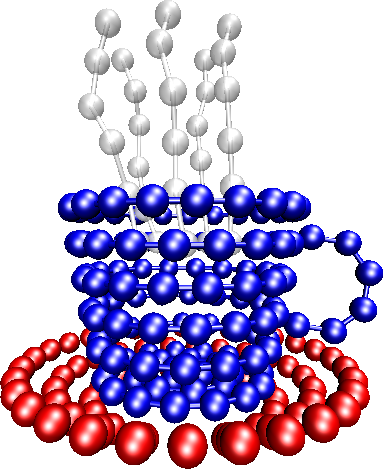
\includegraphics[width=5cm]{logo/transparentbg}
    \end{center}
  }
}

\newtheorem{task}{Task}

\begin{document}
\renewcommand{\d}{\mathrm d}
\subject{ESPResSo Tutorial}
\title{The GPU Electrokinetics method in \ES{}: 
Electroosmotic Flow
} %\author{ Georg Rempfer \thanks{\ttfamily georg@icp.uni-stuttgart.de}}
\date{\today}
\publishers{Institute for Computational Physics, University of Stuttgart}
\maketitle 
\begin{center}
  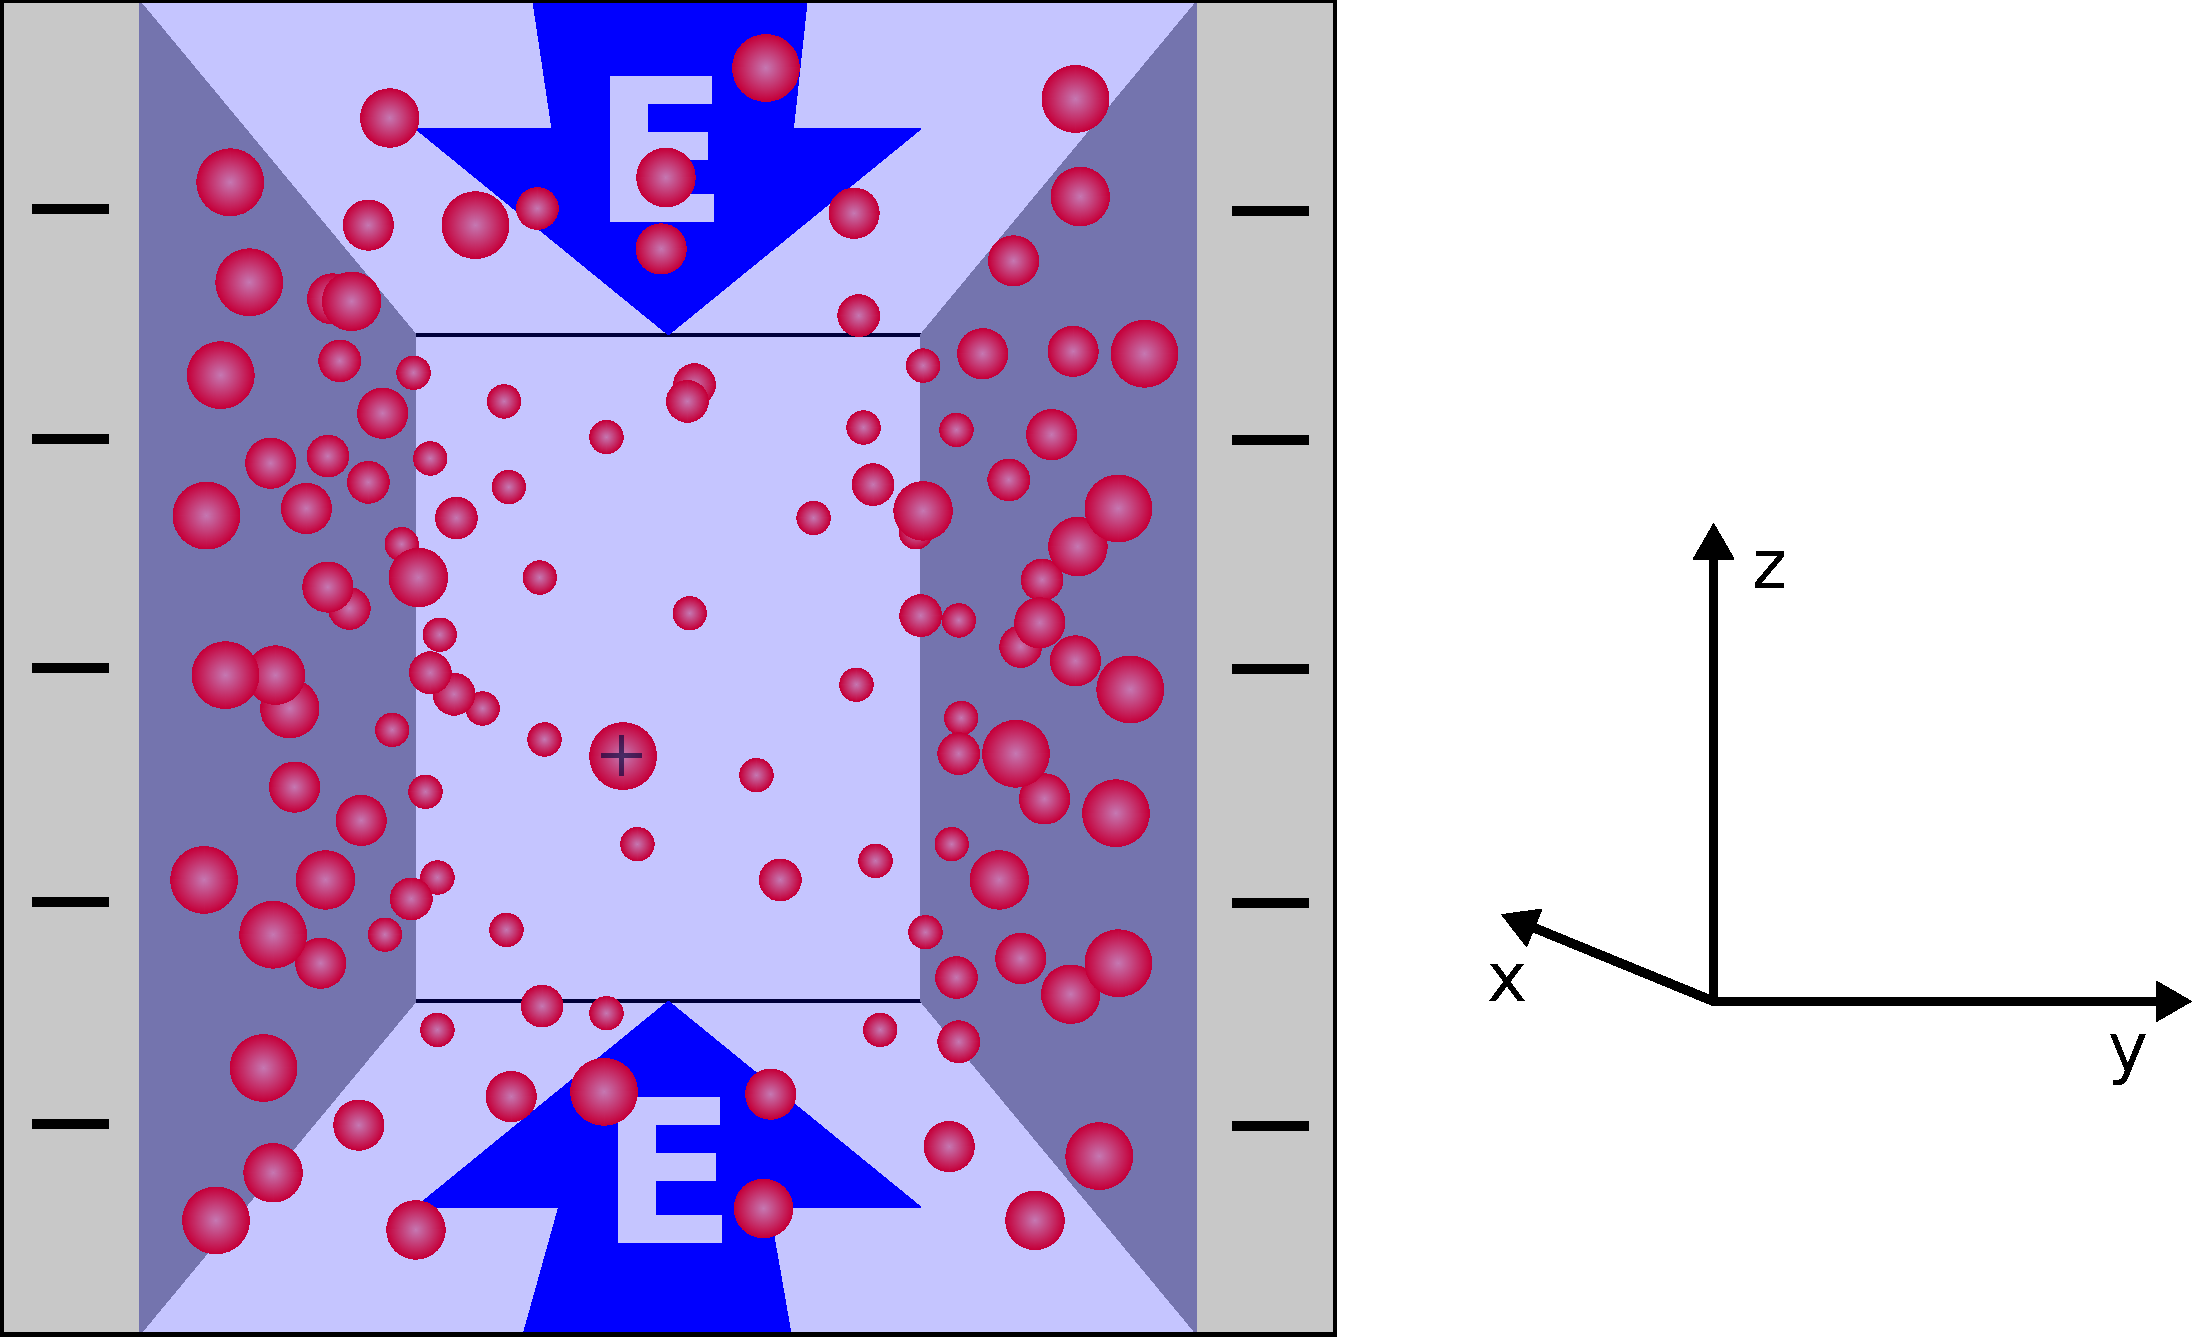
\includegraphics[width=0.7\columnwidth]{figures/schlitzpore_3d.pdf}
\end{center}
\pagebreak
\definecolor{mygray}{gray}{.75}
%\begin{center}
%  \colorbox{mygray}{ 
%\begin{minipage}[h]{13cm}
%  {\bf \large Before you start:}\\
%  With this tutorial you can get started using the Electrokinetics method
%  for scientific applications. We give a brief introduction about the theory
%  and how to use it \ES{}. 
%  We have selected one sample problem for which an analytic solution exists.
%\end{minipage}
%}
%\end{center}

 \tableofcontents
 \pagebreak
  
\section{Introduction}

%\floatingBox{5}{4cm}{Mein Text der in der Box abgebildet werden soll. Mal schauen wie das klappt.} 

In recent years the lattice-Boltzmann method (LBM) has proven itself to be a viable way to introduce hydrodynamic interactions into coarse-grained MD simulations with moderate computational cost. The success of the GPU LBM implementation in \ES{} and similar developments in other software packages created demand for further developments in this area. \ES{} features two such algorithms, namely ELECTROHYDRODYNAMICS, and ELECTROKINETICS (EK). Both of these make use of the LBM and extend it to coarse-grain not only the solvent molecules but also ionic solutes. ELECTROHYDRODYNAMICS does so using a slip layer coupling for charged particles valid in the thin Debye layer (large salt concentration) limit, while EK explicitly treats the ionic solutes in a continuum fashion and is valid for a wide range of salt concentrations.

\subsection*{Tutorial Outline}

To make our first steps using ELECTROKINETICS we will work on one of the few systems for which analytic solutions for the electrokinetic equations exist -- the slip pore geometry with a counterion-only electrolyte. The same slit pore system is also treated in the LBM tutorial, but there, the ionic species were modeled as explicit particles. For this system, the two approaches lead to exactly the same results~\cite{rempfer10a}. Differences are only becoming significant for multivalent ions, very high salt concentrations, and very high surface charges.

This tutorial is divided into three sections. The first section~\ref{sec:theory} introduces the electrokinetic equations and the analytical solution for the slit pore system, while the second section~\ref{sec:simulation} deals exclusively with the simulation, its setup, and the results.

If you already know about simple diffusion-migration-advection equations, continuum electrostatics, and Navier-Stokes, then you can skip the first section.

\pagebreak

% Copyright (C) 2010,2011 The ESPResSo project
%  
% This file is part of ESPResSo.
%   
% ESPResSo is free software: you can redistribute it and/or modify it
% under the terms of the GNU General Public License as published by the
% Free Software Foundation, either version 3 of the License, or (at your
% option) any later version.
%  
% ESPResSo is distributed in the hope that it will be useful, but
% WITHOUT ANY WARRANTY; without even the implied warranty of
% MERCHANTABILITY or FITNESS FOR A PARTICULAR PURPOSE.  See the GNU
% General Public License for more details.
%  
% You should have received a copy of the GNU General Public License
% along with this program.  If not, see <http://www.gnu.org/licenses/>.
%

\chapter{Lattice-Boltzmann}
\label{sec:lb}
\newescommand{lb}

For an implicit treatment of a solvent, \es allows to couple the
molecular dynamics simulation to a Lattice-Boltzmann fluid. The Lattice-
Boltzmann-Method (LBM) is a fast, lattice based method that, in its
``pure'' form, allows to calculate fluid flow in different boundary conditions
of arbitrarily complex geometries. Coupled to molecular dynamics, it allows for 
the computationally efficient inclusion of hydrodynamic interactions into the 
simulation. The implementation of boundary conditions for the LBM is a difficult
 task, a lot of research is still being conducted on this topic. The focus of 
the \es implementation of the LBM is, of course, the coupling to MD and 
therefore available geometries and boundary conditions are somewhat limited 
in comparison to ``pure'' codes. 

Here we restrict the documentation to the interface. For a more detailed
description of the method, please refer to the literature.

\section{Setting up a LB fluid}
\begin{essyntax}
  lbfluid
  \require{2}{\opt{gpu}}
  \require{1 or 2}{\opt{agrid  \var{agrid}}}
  \require{1 or 2}{\opt{dens  \var{density}}}
  \require{1 or 2}{\opt{visc  \var{viscosity}}}
  \require{1 or 2}{\opt{tau  \var{lb\_timestep}}}
  \require{1 or 2}{\opt{bulk_visc  \var{bulk\_viscosity}}}
  \require{1 or 2}{\opt{ext_force  \var{f_x} \var{f_y} \var{f_z}}}
  \require{1 or 2}{\opt{friction   \var{gamma} } }
  \require{1 or 2}{\opt{gamma_odd  \var{gamma\_odd}}}
  \require{1 or 2}{\opt{gamma_even  \var{gamma\_even}}}
  \begin{features}
  \required[1]{LB}
  \required[2]{LB_GPU}
  \end{features}
\end{essyntax}
The \lit{lbfluid} command initializes the fluid with a given
set of parameters. It is also possible to change parameters on the
fly, but this will only rarely be done in practice. Before being able
to use the LBM, it is necessary to set up a box of a desired size. The
parameter \lit{agrid} is used to set the lattice constant of the
fluid, so the size of the box in every direction must be a multiple of
\var{agrid}.

In \es the LB scheme and the MD scheme are not synchronized: In one LB
time step typically several MD steps are performed. This allows to
speed up the simulations and is adjusted with the parameter \var{tau},
the LB timestep.
The parameters \var{dens} and \var{visc} set up the density and
(kinematic) viscosity of the LB fluid in (usual) MD units.  Internally the LB
implementation works with a different set of units: all lengths are
expressed in \var{agrid}, all times in \var{tau} and so on.  Therefore
changing \var{agrid} and \var{tau}, might change the behaviour of the
LB fluid, \eg at boundaries, due to characteristics of the LBM
itself. It should also be noted that the LB nodes are located at 0.5, 1.5, 2.5, etc (in terms of \var{agrid}).
This has important implications for the location of hydrodynamic boundaries which are generally considered
to be halfway between two nodes to first order.
Currently it is not possible to precisely give a parameter set
where reliable results are expected, but we are currently performing a
study on that. Therefore the LBM should \emph{not be used as a black
  box}, but only after a careful check of all parameters that were
applied. 

The parameter \lit{ext_force} allows to apply an external body force
density that is homogeneous over the fluid. It is again to be given in
MD units.  The parameter \lit{bulk_viscosity} allows to tune the bulk
viscosity of the fluid and is given in MD units. In the limit of low
Mach (often also low Reynolds) number the results should be
independent of the bulk viscosity up to a scaling factor. 
It is however known that the values of the viscosity does 
affect the quality of the implemented link-bounce-back method.
\lit{gamma_odd} and
\lit{gamma_even} are the relaxation parameters for the kinetic
modes. Due to their somewhat obscure nature they are to be given
directly in LB units.

Before running a simulation at least the following parameters must be
set up: \lit{agrid}, \lit {dens}, \lit{visc}, \lit{tau},
\lit{friction}. For the other parameters, the following are taken:
\var{bulk\_viscosity}=0, \var{gamma\_odd}=0, \var{gamma\_even}=0,
\var{ f_x} = \var{ f_y} = \var{ f_z} = 0.

\begin{essyntax}
  lbfluid print_interpolated_velocity \var{x} \var{y} \var{z}
\end{essyntax}
This variant returns the velocity at point in countinous space. 
This can make it easier to calculate flow profiles independent of
the lattice constant.

\begin{essyntax}
  lbfluid print \opt{vtk} \var{property} \var{filename}
\end{essyntax}
The print parameter is a feature to simplify visualization. It allows for the 
export of the whole fluid field data into a file with name \var{filename} at 
once. Currently supported values for the parameter \var{property} are boundary 
and velocity. The additional option \lit{vtk} enables export in the vtk format 
which is readable by visualization software such as paraview or mayavi. 
Otherwise gnuplot readable data will be exported.

\begin{essyntax}
  lbfluid save_ascii_checkpoint \var{filename}
  lbfluid save_binary_checkpoint \var{filename}
  lbfluid load_ascii_checkpoint \var{filename}
  lbfluid load_binary_checkpoint \var{filename}
\end{essyntax}
The first two save commands save all of the LB fluid nodes' populations to \var{filename} in ascii or binary format respectively.
The two load commands load the populations from \var{filename}.  This is  useful for restarting a simulation either on the same
machine or a different machine.  Some care should be taken when using the binary format as the format of doubles can depend
on both the computer being used as well as the compiler.  This is currently  only implemented for the cpu version of LB.

\section{LB as a thermostat}
\begin{essyntax}
  thermostat \require{1 or 2}{lb} \var{T}
  \begin{features}
  \required[1]{LB}
  \required[2]{LB_GPU}
  \end{features}
\end{essyntax}
The LBM implementation in \es uses Duenweg's point coupling method
to couple MD particles the LB fluid. This coupling consists
in a frictional force and a random force:
\begin{equation*}
  \vec{F} = -\gamma \left(\vec{v}-\vec{u}\right) + \vec{F}_R.
\end{equation*}
The frictional force tends to decrease the relative velocity
between the fluid and the particle whereas the random forces are chosen
so large that the average kinetic energy per particle corresponds to
the given temperature, according to a fluctuation dissipation theorem.
No other thermostatting mechanism is necessary then. Please any of these
off before starting the LB thermostatting mechanism.

The LBM implementation provides a fully thermalized LB fluid, \ie all
nonconserved modes, including the pressure tensor, fluctuate correctly
according to the given temperature and the relaxation parameters. All
fluctuations can be switched off by setting the temperature to 0.


\section{Reading and setting single lattice nodes}
\begin{essyntax}
  lbnode \var{x} \var{y} \var{z} \alt{print \asep set} \var{args}
  \begin{features}
  \required{LB}
  \end{features}
\end{essyntax}
The \lit{lbnode} command allows to inspect (\lit{print}) and modify
(\lit{set}) single LB nodes.  Note that the indexing in every
direction starts with 0.  For both commands you have to specify what
quantity should be printed
or modified. Print allows the following arguments: \\
\begin{tabular}{p{0.2\columnwidth}p{0.5\columnwidth}}
  \lit{rho}\ & the density (scalar). \\
  \lit{u} & the fluid velocity (three floats: $u_x$, $u_y$, $u_z$) \\
  \lit{pi} & the fluid velocity (six floats: $\Pi_{xx}$, $\Pi_{xy}$, $\Pi_{yy}$, $\Pi_{xz}$,  $\Pi_{yz}$,  $\Pi_{zz}$) \\
  \lit{pi_neq} & the nonequilbrium part of the pressure tensor, components as above. \\
  \lit{pop} & the 19 population (check the order from the source code please). \\
  \lit{boundary} & the flag indicating whether the node is a fluid node ($\lit{boundary}=0$) or a boundary node ($\lit{boundary}\ne 0$). Does not support \lit{set}. Refer to the \lit{lbboundary} command for this functionality.
\end{tabular} \\
Example:
The line
\begin{tclcode}
puts [ lbnode 0 0 0 print u ]
\end{tclcode}
prints the fluid velocity in node 0 0 0 to the screen.  The command
\lit{set} allows to change the density or fluid velocity in a single
node. Setting the other quantities can easily be implemented.
Example:
\begin{tclcode}
puts [ lbnode 0 0 0 set u 0.01 0. 0.]
\end{tclcode}

\section{Setting up boundary conditions}
\begin{essyntax}
  lbboundary \var{shape} \var{shape\_args} \opt{velocity \var{vx} \var{vy} \var{vz}}
  \begin{features}
  \required{LB_BOUNDARIES}
  \end{features}
\end{essyntax}

If nothing else is specified periodic boundary conditions are assumed 
for the LB fluid. The \lit{lbboundary} command allows to set up
other (internal or external) boundaries.

The \lit{lbboundary} command syntax is very close to the
\lit{constraint} syntax, as usually one wants the hydrodynamic
boundary conditions to be shaped similarily to the MD
boundaries. Currently the shapes mentioned above are available and
their syntax exactly follows the syntax of the constraint command. For
example
\begin{tclcode}
  lbboundary wall dist 1.5 normal 1. 0. 0. 
\end{tclcode}
creates a planar boundary condition at distance 1.5 from the origin of
the coordinate system where the half space $x>1.5$ is treated as
normal LB fluid, and the other half space is filled with boundary
nodes.

Intersecting boundaries are in principle possible but must be treated
with care. 
In the current, only partly satisfactory, all nodes that are within at least
one boundary are treated as boundary nodes. Improving this is nontrivial, 
and suggestions are very welcome.

Currently, only the so called ``link-bounce-back'' algorithm for wall
nodes is available. This creates a boundary that is located
approximately midway between the lattice nodes, so in the above
example this corresponds indeed to a boundary at $x=1.5$. Note that
the location of the boundary is unfortunately not independent of the
viscosity. This can \eg be seen when using the sample script
\lit{poisseuille.tcl} with a high viscosity.

The bounce back boundary conditions allow to set velocity at a boundary to a nonzero
value. This allows to create shear flow and boundaries moving relative to 
each other. This could be a fixed sphere in a channel moving at a finite speed -- 
corresponding to the galilei-transform of a moving sphere in a fixed channel.
The velocity boundary conditions are implemented according to \cite{succi01a}
eq.~12.58. Using this implementation as a blueprint for the boundary treatment 
an implementation of the Ladd-Coupling should be relatively straightforward.

\begin{essyntax}
  lbboundary force \opt{ \var{n_{boundary}}}
  \begin{features}
  \required{LB_BOUNDARIES}
  \end{features}
\end{essyntax}
This variant prints out the force on boundary number \lit{n_boundary}.

\section{Choosing between the GPU and CPU implementations}
\begin{essyntax}
  \variant{1} lbfluid cpu
  \variant{2} lbfluid gpu
  \begin{features}
    \required[1]{LB}
    \required[2]{LB_GPU}
  \end{features}
\end{essyntax}

A very recent development is an implementation of the LBM for NVIDIA
GPUs using the CUDA framework.  On CUDA-supporting machines this can
be activated by configuring with \lit{configure
  --with-cuda=/path/to/cuda} and activating the feature \lit{LB_GPU}.
Within the \es-Tcl-script, the \lit{lbfluid} command can be used to
choose between the CPU and GPU implementations of the
Lattice-Boltzmann algorithm, for further information on CUDA support
see section~\ref{sec:cuda}.

Variant \variant{1} is the default and turns on the standard CPU
implementation of the Lattice-Boltzmann fluid, while variant
\variant{2} turns on the GPU implementation, implying that all
following LB-related commands are executed on the GPU.

Currently only a subset of the CPU commands are available for the GPU
implementation.  For boundary conditions analogous to the CPU
implementation, the feature \lit{LB_BOUNDARIES_GPU} has to be
activated.

\section{Electrohydrodynamics}

\begin{essyntax}
  setmd mu_E \var{\mu E_x} \var{\mu E_y} \var{\mu E_z}
  \begin{features}
    \required{LB}
    \required{LB_ELECTROHYDRODYNAMICS}
  \end{features}
\end{essyntax}

If the feature \lit{LB_ELECTROHYDRODYNAMICS} is activated, the
(non-GPU) Lattice Boltzmann Code can be used to implicitely model
surrounding salt ions in an external electric field by having the
charged particles create flow.

For that to work, you need to set the electrophoretic mobility
(multiplied by the external $E$-field) $\mu E$ in all 3 dimensions for
your system. The three given parameters are float values and should,
for a meaningful system, be less than $1.0$.

For more information on this method and how it works, read the
publication~\cite{hickey10a}.

%%% Local Variables:
%%% mode: latex
%%% TeX-master: "ug"
%%% End:



\section{The LB interface in \ES{}}
\ES{} features two virtually independent implementations of LB. One implementation
uses CPUs and one uses a GPU to perform the computational work. For this, we
provide two actor classes \texttt{LBFluid} and \texttt{LBFluid\_GPU} with the
module \texttt{espressomd.lb}, as well as the optional \texttt{LBBoundary} class
found in \texttt{espressomd.lbboundaries}.

The LB lattice is a cubic lattice, with a lattice constant \texttt{agrid} that
is the same in all spacial directions. The chosen box length must be an integer multiple
of \texttt{agrid}. The LB lattice is shifted by 0.5 \texttt{agrid} in all directions: the node
with integer coordinates $\left(0,0,0\right)$ is located at
$\left(0.5a,0.5a,0.5a\right)$.
The LB scheme and the MD scheme are not synchronized: In one
LB time step, several MD steps may be performed. This allows to speed
up the simulations and is adjusted with the parameter \texttt{tau}.
The LB parameter \texttt{tau} must be an integer multiple of the MD timestep.

Even if MD features are not used, the System parameters \texttt{skin} and
\texttt{time\_step} must be set. LB steps are performed 
in regular intervals, such that the timestep $\tau$ for LB is recovered. 

Important Notice: All commands of the LB interface use
MD units. This is convenient, as e.g. a particular 
viscosity can be set and the LB time step can be changed without
altering the viscosity. On the other hand this is a source
of a plethora of mistakes: The LBM is only reliable in a certain 
range of parameters (in LB units) and the unit conversion
may take some of them far out of this range. So note that you always
have to assure that you are not messing with that!

One brief example: a certain velocity may be 10 in MD units.
If the LB time step is 0.1 in MD units, and the lattice constant
is 1, then it corresponds to a velocity of $1\ \frac{a}{\tau}$ in LB units.
This is the maximum velocity of the discrete velocity set and therefore
causes numerical instabilities like negative populations.

\subsection*{The \texttt{LBFluid} class}
The \texttt{LBFluid} class provides an interface to the LB-Method in the \ES{}
core. When initializing an object, one can pass the aforementioned parameters
as keyword arguments. Parameters are given in MD units. The available keyword
arguments are:



\vspace{0,2cm}
\begin{tabular}{p{0.2\columnwidth}p{0.5\columnwidth}}
\texttt{dens} & The density of the fluid.\\
\texttt{agrid} & The lattice constant of the fluid. It is used to determine the number of LB nodes 
per direction from \texttt{box\_l}. {\em They have to be compatible.} \\
\texttt{visc} & The kinematic viscosity \\
  \texttt{tau} & The time step of LB. It has to be an integer multiple of
  \texttt{System.time\_step}. \\
\texttt{fric} & The friction coefficient $\gamma$ for the coupling scheme. \\
\texttt{ext\_force} & An external force applied to every node. This is given as
a list, tuple or array with three components.%\\
%\texttt{gamma\_odd} & Relaxation parameter for the odd kinetic modes. \\
%\texttt{gamma\_even} & Relaxation parameter for the even kinetic modes.
\end{tabular}\\ 
\vspace{0,2cm}

Using these arguments, one can initialize an LBFluid object. This object then
needs to be added to the systen's actor list. The code below provides a minimum
example.
\vspace{0,2cm}
\begin{pypresso}
  from espressomd import system, lb

  # initialize the System and set the necessary MD parameters for LB.
  s = system.System()
  s.box_l = [31, 41, 59]
  s.time_step = 0.01
  s.cell_system.skin = 0.4

  # Initialize and LBFluid with the minimum set of valid parameters.
  lbf = lb.LBFluid(agrid = 1, dens = 10, visc = .1, tau = 0.01)
  # Activate the LB by adding it to the System's actor list.
  s.actor.add(lbf)
\end{pypresso}
\vspace{0,2cm}
Note: The same applies for the class \texttt{LBFluid\_GPU}.

\subsection*{Sampling data from a node}
The \texttt{LBFluid} class also provides a set of methods which can be used to
sample data from the fluid nodes. For example 
\vspace{0,2cm}
\begin{pypresso}
  lbf.lbnode_get_node_xxxx([X,Y,Z])
\end{pypresso}
\vspace{0,2cm}
returns the propert xxxx of the node with $(X,Y,Z)$ coordinates. Note that the
indexing in every direction starts with 0. The possible properties are:
\vspace{0,8cm}
\begin{tabular}{p{0.2\columnwidth}p{0.5\columnwidth}}
  \texttt{velocity} & the fluid velocity (list of three floats) \\
  \texttt{pi} & the stress tensor (list of six floats: $\Pi_{xx}$, $\Pi_{xy}$, $\Pi_{yy}$, $\Pi_{xz}$,  $\Pi_{yz}$,  $\Pi_{zz}$) \\
  \texttt{pi\_neq} & the nonequilbrium part of the stress tensor, components as above. \\
  \texttt{pop} & the 19 populations of the D3Q19 lattice.\\
  \texttt{boundary} & The boundary index.\\
  \texttt{density}\ & the local density. 
\end{tabular} \\
\vspace{0,8cm}

\subsection*{The \texttt{LBBoundary} class}
The \texttt{LBBoundary} class represents a boundary on the \texttt{LBFluid}
lattice. It is dependent on the classes of the module $\texttt{espressomd.shapes}$ as it
derives its geometry from them. For the initialization, the arguments
\texttt{shape} and \texttt{velocity} are supported. The \texttt{shape} argument
takes an object from the \texttt{shapes} module and the \texttt{velocity}
argument expects a list, tuple or array containing 3 floats. Setting the
\texttt{velocity} will results in a slip boundary condition.

Note that the boundaries are not constructed
through the periodic boundary. If, for example, one would set a sphere with
its center in one of the corner of the boxes, a sphere fragment will be
generated. To avoid this, make sure the sphere, or any other boundary, fits
inside the original box.

This part of the LB implementation is still experimental,
so please tell us about your experience with it. In general even the simple case of no-slip
boundary is still an important research topic in the lb community and in combination with
point particle coupling not much experience exists. This means: Do research on that topic, play
around with parameters and figure out what happens. 

Boundaries are initialized by passing a shape object to the \texttt{LBBoundary}
class. One way to initialize a wall is:
\begin{pypresso}
  from espressomd import lbboundaries
  wall = lbboundaries.LBBoundary(shape=shapes.Wall(normal=[1,0,0],
                                                   dist=1),
                                 velocity = [0, 0, 0.01])
  s.lbboundaries.add(wall)
\end{pypresso}
Note that all used variables are inherited from previous examples. This will
create a wall a surface normal of $(1,0,0)$ at a distance of $1$ from the origin
of the coordinate system in direction of the normal vector. The wall exhibits a
slip boundary condition with a velocity of $(0,0,0.01)$. For the a no-slip
condition, leave out the velocity argument or set it so zero. Please refer to the
user guide for a complete list of constraints.

Currently only the so called \emph{link bounce back} method is implemented, where the effective
hydrodynamic boundary is located midway between two nodes. This is the simplest and yet a 
rather effective approach for boundary implementation. Using the shape objects
distance function, the nodes determine once during initialisation whether they
are boundary or fluid nodes.


\section{Drag force on objects}
As a first test, we measure the drag force on different objects in a simulation
box. Under low Reynolds number conditions, an object with velocity $\vec{v}$
experiences a drag force $\vec{F}_\text{D}$ proportional to the velocity:
\begin{align*}
	\vec{F}_\text{D}=-\gamma\vec{v},
\end{align*}
where $\gamma$ is denoted the friction coefficient. In general $\gamma$ is a
tensor thus the drag force is generally not parallel to the velocity. For
spherical particles the drag force is given by Stokes' law:
\begin{align*}
	\vec{F}_\text{D}=-6\pi\eta a\vec{v},
\end{align*}
where $a$ is the radius of the sphere.

In this task you will measure the drag force on falling objects with LB and
\ES{}. In the sample script {\tt lb\_stokes\_force.tcl} a spherical object at rest
is centered in a square channel. Bounce back boundary conditions are assumed on
the sphere. At the channel boundary the velocity is fixed by using appropriate
boundary conditions. Within a few hundred or thousand  integration steps a
steady state develops and the force on the sphere converges.

\subsection*{Radius dependence of the drag force}
Measure the drag force for three different input radii of the sphere. How good
is the agreement with Stokes' law? Calculate an effective radius from Stokes'
law and the drag force measured in the simulation. Is there a clear relation to
the input radius? Remember how the bounce back boundary condition work and how
good spheres can be represented by them.

\subsection*{Visualization of the flow field}
The script produces {\tt vtk} files of the flow field. Visualize the flow field
with {\tt paraview}. Open {\tt paraview} by typing it on the command line. Make
sure you are in the folder where the files are located. So the agenda is:
\begin{itemize}
	\item Click in the menu {\tt File}, {\tt Open...}
	\item Choose the files with flow field {\tt fluid...vtk}
	\item Click {\tt Apply}
	\item Add a stream tracer filter {\tt Filters}, {\tt Alphabetical}, {\tt
		Stream tracer}
	\item Change the seed type from {\tt point source} to {\tt high resolution
		line source}
	\item Click {\tt Apply}
	\item Rotate the visualization box to see the stream lines.
	\item Use the play button in the bar below the menu bar to show the time
		evolution.
\end{itemize}

\subsection*{System size dependence}
Measure the drag force for a fixed radius but varying system size. Does the drag
force increase of decrease with the system size? Can you find a qualitative
explanation?
\end{align*}

\section{Polymer Diffusion}
In these exercises we want to use the LBM-MD-Hybrid to reproduce a classic
result of polymer physics: The dependence of the diffusion coefficient
of a polymer on its chain length. If no hydrodynamic interactions
are present, one expects a scaling law $D \propto N^{-1}$ and if 
they are present, a scaling law $D \propto N^{-\nu}$ is expected. 
Here $\nu$ is the Flory exponent that plays a very prominent role
in polymer physics. It has a value of $\sim 3/5$ in good solvent
conditions in 3D. Discussions of these scaling laws can be found
in polymer physics textbooks like \cite{degennes79a, doi96a, rubinstein03a}.


The reason for the different scaling law is the following:
When being transported, every monomer creates a flow field that follows
the direction of its motion. This flow field makes it easier 
for other monomers to follow its motion. This makes a polymer
long enough diffuse more like compact object including the fluid
inside it, although it does not have clear boundaries. It can be shown 
that its motion can be described by its hydrodynamic radius. It is defined 
as:
\begin{equation}
  \langle \frac{1}{R_h} \rangle = \langle \frac{1}{N^2}\sum_{i\neq j} \frac{1}{\left| r_i - r_j \right|} \rangle
\end{equation}
This hydrodynamic radius exhibits the scaling law  $R_h \propto N^{\nu}$
and the diffusion coefficient of long polymer is proportional to its inverse.
For shorter polymers there is a transition region. It can be described
by the Kirkwood-Zimm model:
\begin{equation}
  D=\frac{D_0}{N} + \frac{k_B T}{6 \pi \eta } \langle \frac{1}{R_h} \rangle
\end{equation}
Here $D_0$ is the monomer diffusion coefficient and $\eta$ the 
viscosity of the fluid. For a finite system size the second part of the
diffusion is subject of a $1/L$ finite size effect, because
hydrodynamic interactions are proportional to the inverse
distance and thus long ranged. It can be taken into account
by a correction:
\begin{equation}
  D=\frac{D_0}{N} + \frac{k_B T}{6 \pi \eta } \langle \frac{1}{R_h} \rangle \left( 1- \langle\frac{R_h}{L} \rangle \right)
  \label{kirkwood}
\end{equation}
It is quite difficult to prove this formula with good accuracy. It will 
need quite some computer time and a careful analysis. So please don't be
too disappointed if you don't manage to do so.


We want to determine the diffusion coefficient from the mean square
distance that a particle travels in the time $t$. For large $t$ it is
be proportional to the time and the diffusion coefficient occurs as 
prefactor: 
\begin{equation}
  \frac{\partial \langle r^2 \left(t\right)\rangle}{\partial t} = 2 d D. 
  \label{eq:msd}
\end{equation}
Here $d$ denotes the dimensionality of the system, in our case 3.
This equation can be found in virtually any simulation textbook, like
\cite{frenkel02b}.
We will therefore set up a polymer in an LB fluid, simulate for an appropriate
amount of time, calculate the mean square displacement as a function of
time and obtain the diffusion coefficient from a linear fit. However
we make a couple of steps in between and divide the full problem into 
subproblems that allow to (hopefully) fully understand the process.

\subsection{Step 1: Diffusion of a single particle}
Our first step is to investigate the diffusion of a single particle
that is coupled to an LB fluid by the point coupling method.
Take a look at the script \texttt{single\_particle\_diffusion.py}.
The script takes the LB-friction coefficient as an argument. Start with
an friction coefficient of 1.0:
{\vspace{0,2cm}\small
\begin{lstlisting}[numbers=none]
/path/to/pypresso single_particle_diffusion.py 1.0
\end{lstlisting}
\vspace{0,2cm}
}

In this script an LB fluid and a single particle are created and
thermalized. 
The random forces on the particle and
within the LB fluid will cause the particle to move. The mean squared
displacement is calculated during the simulation via a multiple-tau correlator. 
Run the simulation script and plot the output data \texttt{msd\_1.0.dat}. To
load the file into a numpy array, one can use \texttt{numpy.loadtxt}.
Zoom in on the origin of the plot. What do you see for short times? What do you
see on a longer time scale? Produce a double-logarithmic plot to assess the power
law.
\begin{figure}[h]
  \begin{center}
	  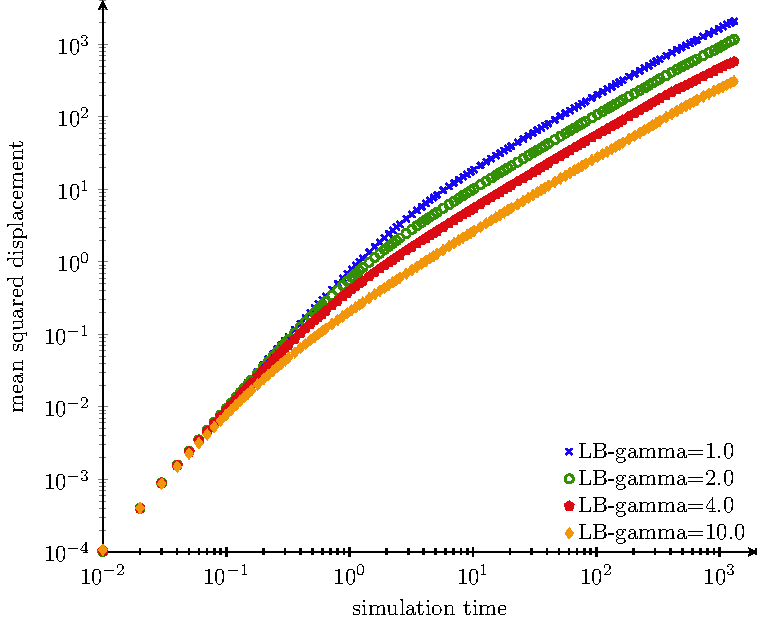
\includegraphics{figures/diffusion/msd.pdf}
  \end{center}
  \caption{Mean squared displacement of a single particle for different values
  of LB friction coefficient.}
\end{figure}

Can you give an explanation for the quadratic time dependency for short
times?
Use the function \texttt{curve\_fit} from the module \texttt{scipy.optimize} to
produce a fit for the linear regime and determine the diffusion coefficient.

%The file \lstinline|energy.dat| contains the kinetic energy of the
%particle as a function of the elapsed simulation time. Investigate
%it, by plotting it with gnuplot. Calculate the average value of 
%the kinetic energy e.g. by fitting a constant function with gnuplot.
%What value would you expect from a working thermostat?

Run the simulation again with different values for the friction
coefficient, e.g. 1. 2. 4. 10. Calculate the diffusion
coefficient for all cases and plot them as a function of $\gamma$. What relation
do you observe?

%The tiny helper script \lstinline|fit_lin.sh| 
%(with argument \lstinline|msd_pos.dat|)
%will help you with that. It contains
%a (quite ugly) gnuplot one-liner that does the fitting and just
%returns the slope. The fit is performed in the range 5 to 40 that
%has proved to work good for runs of $\sim 100000$ steps. You have to 
%modify the script to change that range.
%Is there any difference between the
%friction coefficient that you put in, and the diffusion coefficient
%you obtain?

%\section{Step 3: The long time tail of the velocity autocorrelation function}
%Should we do anything here?

\subsection{Step 2: Diffusion of a polymer}
One of the typical applications of \ES{} is the simulation of polymer chains 
with a bead-spring-model. For this we need a repulsive interaction
between all beads, for which one usually takes a shifted and truncated
Lennard-Jones (so called Weeks-Chandler-Anderson) interaction, 
and additionally a bonded interaction between 
adjacent beads to hold the polymer together. You have already learned
that the command
{\vspace{0,2cm}\small
\begin{pypresso}
  s.non_bonded_inter[0,0].lennard_jones.set_params(
      epsilon = 1.0, sigma = 1.0,
      shift = 0.25, cutof = 1.226)
\end{pypresso}\vspace{0,2cm}
}
creates a Lennard-Jones interaction with $\varepsilon=1.$, $\sigma=1.$,
$r_\text{cut} = 1.125$ and $\varepsilon_\text{shift}=0.25$ between particles
of type 0, which is the desired 
repulsive interaction. The command
{\vspace{0,2cm}\small
\begin{pypresso}
  from espressomd import interactions
  fene = interactions.FeneBond(k = 7,d_r_max = 2)
\end{pypresso}
\vspace{0,2cm}
}
creates a \texttt{FeneBond} object (see \ES{} manual for the details). Still \ES{}
does not know between which beads this interaction should be applied.
This can be either be specified explicitly or done with the \texttt{polymer}
module. This creates a given number of beads, links them with the given
bonded interaction and places them following a certain algorithm. We will
use the pruned self-avoiding walk: The monomers are set according 
to a pruned self-avoiding walk (in 3D) with a
fixed distance between adjacent bead positions. The syntax is:
{\vspace{0,2cm}\small
\begin{pypresso}
  from espressomd import polymer
  # mpc: monomers per chain
  mpc = 30
  poly = system.polymer(N_P=1, MPC = mpc, bond_id=fene._bond_id,
                        bond_length = 1)
\end{pypresso}
\vspace{0,2cm}
}
Using a random walk to create a polymer causes trouble: The random walk may 
cross itself (or closely approach itself) and the LJ potential is very
steep. This would raise the potential energy enormously and would make
the monomers shoot through the simulation box. The pruned self-avoiding
walk should prevent that, but to be sure
we perform some MD steps with a capped LJ potential, this means 
forces above a certain threshold will be set to the threshold in order to prevent
the system from exploding. To see how this is done, look at the script 
\texttt{polymer\_diffusion.py}.
It contains a quite long warmup command so that also longer polymers
are possible. You can probably make it shorter.

It is called in the following way:
{\vspace{0,2cm}\small
\begin{lstlisting}[numbers=none]
/path/to/pypresso polymer_diffusion.py $N_monomers  
\end{lstlisting}\vspace{0,2cm}
}
This allows to quickly change the number of monomers without editing 
the script.
For the warmup a Langevin thermostat is used to keep the temperature constant.
Furthermore we want to compute the diffusion constant of the polymer for
different numbers of monomers. For this purpose we can again use the multiple
tau correlator. Have a look at the \ES{} -script for the single particle diffusion
and add the adapted commands for the polymer. Find out how many integration steps are
necessary to capture the long-time diffusion regime of the polymer. The script
already computes the time averaged hydrodynamic radius and stores it in a file
\texttt{rh\_nom\_xx.dat} where \texttt{xx} is the number of monomers.

Run the script for different numbers of monomers and determine the evolution of
the diffusion coefficient as a function of the chain length. Compare the results
of your \ES{} simulations with the given Kirkwood-Zimm formula
(eq.~\ref{kirkwood}). 

%\section{Electro-osmotic flow in a slit pore}
%Electro-osmotic flow (EOF) is the motion of water (or another liquid)
%induced by an electric field. It can occur e.g. in porous media,
%in synthetic capillaries and in vicinity of charged surfaces.
%Charged objects in an electrolyte solution attract ions of one
%species and repel ions of the other species, which gives rise
%to a net charge density in its neighbourhood. If an external
%electric field is applied, these ions are accelerated in the direction
%of the electric field (or oppositely if negatively charged) which
%causes also an acceleration of the surrounding water. In regions
%with zero net charge, the force on the fluid exerted by both ion
%species cancels, thus charged interfaces are necessary.
%
%Conceptually electro-osmotic flow is closely related to electrophoresis,
%where a charged object (e.g. a polyelectrolyte) is moved by an
%electric field and the surrounding counterions create a flow field
%in the opposite direction. 
%
%In this exercise the electrokinetic equations, that allow for a classical
%description of the phenomenon, are introduced and you will learn
%how to simulate this effect with \ES{} with the LBM. The special case of
%planar charged walls in the regime of low salt concentration can
%be solved analytically and you will see that we can reproduce the
%classical results quite well, but you will also learn about the
%deficiencies of both approaches. We will concentrate on the case
%where only one species of ions (counterions) is present. The generalization
%to multiple species however is straightforward.
%
%\subsection{The electrokinetic equations}
%We want to describe a system in which ions can diffuse under an
%applied field embedded in a fluid. We therefore assume that a 
%linear convection diffusion equation is valid:
%\begin{align*}
%		\vec j &=-D\nabla\rho-\rho\left(\mu z e \nabla\Phi+\vec u\right),
%\end{align*}
%
%Here $\vec{j}$ corresponds to the ion flux density, $D$ corresponds 
%to the diffusion coefficient of the ions,
%$\rho$ to their concentration, $\mu$ to their (electrophoretic)
%mobility, $z$ the valency, $\vec{E}$ to the local electric field and $\vec{u}$
%to the fluid velocity.
%
%We assume that the fluid fulfills the incompressible Navier-Stokes equation.
%The term $\rho z e \vec{E}$ appears as source term due
%to the acceleration of the fluid caused by the ions. 
%In the limit of small Reynolds numbers we can leave out
%the convection term and reduce to the Stokes equation.
%\begin{equation}
%  \eta \Delta \vec{u} = \vec{\nabla} p - \rho z e \vec{E}
%\end{equation}
%Here we have assumed that the system reaches a steady
%state and therefore the time derivative was dropped.
%The incompressibility (=continuity) equation holds:
%\begin{equation}
%  \vec{\nabla} \cdot \vec{u} = 0
%\end{equation}
%For the electrostatic potential we make the following
%mean field approximation: The electric potential is 
%caused not by single ions, but their density. This means
%every ion is not exposed to the instantaneous electrostatic potential
%but the smeared out potential of all other ions. Then the Poisson
%equation reads as:
%\begin{equation}
%  \Delta \Phi = -\rho z e/\varepsilon
%  \label{asdf}
%\end{equation}
%We will later
%see that this approximation is avoided in a molecular dynamics simulation
%of explicit ions.
%
%This set of coupled partial differential equations is called
%the electrokinetic equations. In general the solution is difficult,
%but the planar geometry will allow us to find an analytical 
%solution.
%
%\subsection{The slit pore geometry}
%We want to investigate the simplest case where EOF occurs:
%The flow of water through the volume between two parallel
%charged planes in the $xy$-plane. We assume that the planes are infinitely
%extended in the directions parallel to the plane and that
%the number of ions exactly cancels the charge of both planes
%and that the external electric field is exerted in $x$ direction
%and that the position of the planes is at $x=\pm l/2$.
%
%We assume that all quantities do not change in $y$ and $z$ directions
%because of translational invariance (the great advantage of our geometry)
%and drop all derivatives with respect to it. The only exception
%is the electrostatic potential which we assume to decay linearly in
%$y$-direction due to an external field. 
%
%
%Due to continuity in $x$-direction and translational invariance resp.
%symmetry the fluid velocity and flux density in x direction must be zero and we can 
%write down the Poisson equation and the diffusion equation in 
%$x$ direction:
%\begin{align}
%  \partial^2_x \Phi &= -\rho z e/\varepsilon \\
%	0 &=-D\partial_x\rho-\rho\mu z e \partial_x\Phi
%\end{align}
%This significantly smaller set of equations corresponds
%to the 1D Poisson-Boltzmann equation. It can be solved
%using the Ansatz:
%\begin{equation}
%  \rho = c \exp\left(-\frac{z e \Phi}{k_B T}\right)
%\end{equation}
%Then one obtains a single ordinary differential
%equation that has to be solved under the boundary 
%condition that the walls bear a charge density $\sigma$,
%thus electric field jumps at $x=\pm l/2$. This
%yields:
%\begin{align*}
%		\rho(y)=\frac{\varepsilon\,C^2}{2 k_B T}\cdot\frac 1 {\cos^2\left(\frac{qC}{2k_B T}\cdot y\right)},\quad \left|\frac{qC}{2k_B T}\cdot y\right|<\frac\pi 2\,.
%	\end{align*}
%Here the parameter $C$ has to fulfill the following transcendental
%equation:
%	\begin{align*}
%		C\cdot\tan\left(\frac{qd}{4k_B T}\cdot C\right)=-\frac\sigma\varepsilon,\quad 0\le C<\frac{\pi k_B T}{2d|q|}\,.
%	\end{align*}
%Now this charge density can be included in the Stokes equation
%and one can obtain the fluid profile from integrating twice
%and choosing the integration constanst so that $\vec u=0$ is fulfilled
%at $x=\pm l/2$:
%	\begin{align*}
%		u_y(x)&=\frac{2E\varepsilon k_B T}{\eta q}\cdot\left\{\log\left[\cos\left(\frac{qC}{2k_B T}\cdot x\right)\right]-\log\left[\cos\left(\frac{dqC}{4k_B T}\right)\right]\right\},\\
%	\end{align*}
%Obtaining the particle flux profile is the easy:
%\begin{equation}
%  j_y / \rho = \mu E + u_y.
%\end{equation}
%
%Before simulating the full system, we make two steps in between, because
%we need to know how to have walls in an \ES{} simulation. First we want
%to simulate Poisseuille flow, the famous parabolic flow profile, in a slit
%geometry and then we want to simulate particles between two walls. Finally
%we combine it all to simulate the full system.

\section{Poiseuille flow \ES{}}
Poisseuille flow is the flow through a pipe or (in our case) a slit
under a homogenous force density, e.g. gravity. In the limit of small Reynolds
numbers, the flow can be described with the Stokes equation. 
We assume the slit being infinitely extended in $y$ and $z$ 
direction and a force density $f$ on the fluid 
in $y$ direction. No slip-boundary conditions  (i.e. $\vec{u}=0$)
are located at $z = \pm l/2$.
Assuming invariance in $y$ and $z$ direction and a steady state 
the Stokes equation is simplified to:
\begin{equation}
  \eta \partial_x^2 u_y = f
\end{equation}
where $f$ denotes the force density and $\eta$ the dynamic viscosity.
This can be integrated twice and the integration constants are chosen
so that $u_y=0$ at $z = \pm l/2$ and we obtain:
\begin{equation}
  u_y = \frac{f}{2\eta} \left(l^2/4-x^2\right)
\end{equation}
With that knowledge investigate the script \texttt{poisseuille.py}.
Note the use of the \texttt{lbboundaries} module. Two walls are created
with normal vectors $\left(\pm 1, 0, 0 \right)$. An external force
is applied to every node. After 5000 LB updates the steady state should
be reached.

Task: Write a loop that prints the fluid velocity at the nodes (0,0,0) to (16,0,0)
and the node position to a file. Use the \texttt{lbf.lbnode\_get\_node\_velocity()}
method for that. Hint: to write 
to a file, first open a file and then use the \texttt{write()} method to write 
into it. Do not forget to close the file afterwards. Example:
\vspace{ 0,2cm}
\begin{pypresso}[numbers=none]
f = open("file.dat", "w")
f.write("Hello world!\n")
f.close()
\end{pypresso}
\vspace{ 0,2cm}
Use the data to fit a parabolic function. Can you confirm the analytic solution?
\begin{figure}[h]
  \begin{center}
    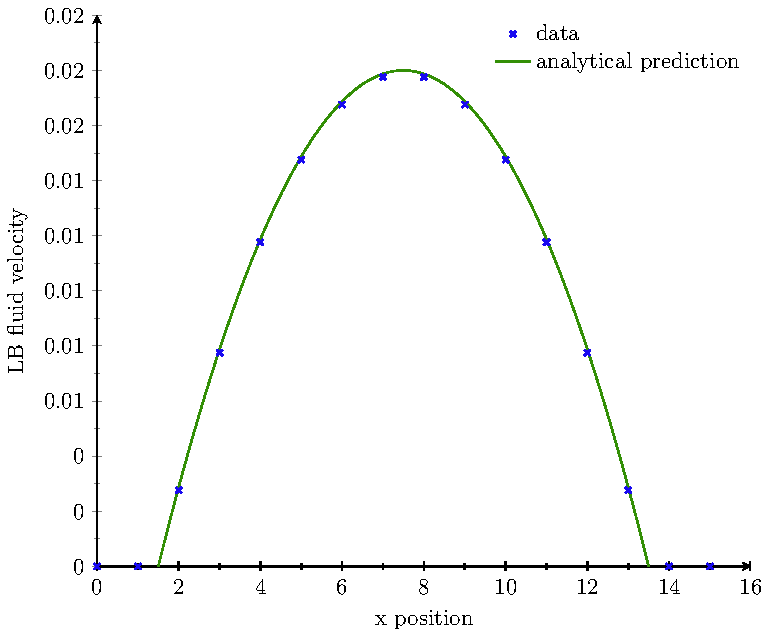
\includegraphics{figures/poiseuille/poiseuille.pdf}
  \end{center}
  \caption{Poisseuille Flow in a slit Geometry.}
\end{figure}

%\subsection{Constraints in \ES{}}
%The \lstinline|constraint| command of \ES{} creates walls in the system.
%They have a particular ``particle'' type and interact with the particles
%present in the system with the potential defined 
%between them. This means the distance
%of every particle to the constraint is calculated and used as the distance 
%in the interaction potential.
%
%To set up a planar channel like the LB channel before one would use the commands:
%\begin{lstlisting}[numbers=none]
%constraint wall dist 0.5 normal 1. 0. 0. type 1
%constraint wall dist -8.5 normal -1. 0. 0. type 1
%inter 0 1 lennard-jones 1. 1. 1.225 0.25 0
%\end{lstlisting}
%This wall is felt only by particles of type 0 and has an effective width
%of 6, as the potential goes steeply up at positions $x=1.5$ and $x=7.5$.
%
%The syntax of the wall constraint looks weird at first, because a negative
%distance from the origin (first argument) is given, but the idea is that
%this distance times the normal vector is a point of the plane. For inclined
%walls this syntax is more easy to understand.
%
%\ES{} complains every time a particle penetrates the wall, as it does not
%expect the particles to do so. This complaint should be taken serious, because
%that means the particle has overcome LJ potential barrier, which is physically
%impossible. This usually tells you to reduce the applied time step.
%
%To set up a system we have, of course to make sure, that our initial
%configuration obeys the constraints. The easiest thing is to 
%generate particle positions randomly and check if it obeys the constraint.
%If not we repeat this process
%for every particle until a configuration is found, that
%is within the allowed range. Look at the script \lstinline|boundaries.tcl|
%and see how that is solved. What does the script do?
%Introduce an LB fluid with planar walls boundaries at 2.5 and 12.5. 
%\subsection{Simulating EOF in \ES{}}
%The last thing that is missing for the simulation of EOF is
%how to create a charged wall. This can be done with
%particles, using the \lstinline|fix| command. The command
%\begin{lstlisting}[numbers=none]
%part 0 pos 1. 1. 1. q 1. fix 1 1 1
%\end{lstlisting}
%create a particle at the position $\left(1,1,1\right)$ with
%charge 1 that is fixed in all the spacial dimensions.
%
%In \lstinline|eof.tcl| two walls are created. Now use the material
%from the other two scripts to run the final system.
%We want to obtain a 10 Nanometer wide channel centered
%$x=7.5$
%\begin{enumerate}
%  \item Create constraints at $x=1.5$ and $x=13.5$ and create 
%    a particle-wall interaction. How can you assure that the 
%    particles creating the wall charges are not affected by 
%    interaction potential?
%  \item
%Use the particle
%creation method from \lstinline|boundaries.tcl| to
%create particles in the system. Create a repulsive potential between them.
%  \item
%Charge the particles so that
%the overall system is neutral. 
%  \item Add an electrostatic interaction with a Bjerrum length 
%    of 0.7 (the room temperature Bjerrum length of water in nanometer).
%  \item First do not exert an external force on the particles.
%       Use a Langevin thermostat to bring the system to equilibrium.
%       It will take some time for the ions to move towards the charged
%       walls. You can use vmd to look at the process.
%  \item
%	  Use the density profile method from {\tt boundaries.tcl}
%       to determine the ion concentration profile. How many samples
%       do you need to get a reasonable concentration profile?
%   \item
%     Plot the concentration profile with gnuplot. Compare with the
%     the Poisson-Boltzmann result. 
%   \item 
%     Introduce an LB fluid with planar walls boundaries at 2.5 and 12.5. 
%     Do not forget to remove the
%	 external force if you copy\&paste from {\tt poisseuille.tcl}.
%   \item 
%     Add an external force of 0.1 to all particles that do not form the
%     charged wall in $y$-direction. Now run the system for enough time
%     steps to get a good flux and velocity profile.
%   \item 
%     Finally calculate the velocity profile. You will have to 
%     average over several steps. Keep in mind that number crunching
%     with tcl is slow and that you will not need to average over too 
%     many samples.
%   \item 
%     Compare the flux and velocity profiles with the result from
%     theory. Do they agree?
%   \item
%     Now increase the charge density on the walls. Can you observe differences
%     between theory and Computer simulations? They will likely be caused
%     by the fact, that MD simulations of explicit ions automatically
%     take into account ion correlations and the effect of the finite size
%     of ions.
%\end{enumerate}
%Following this list should in principle enable you to simulate the system. However
%we have figured out that quite some traps are on the way to the full system. You might
%have to make warmup steps in between, play with the time step and so on until your
%simulation script is really stable. If something happens, make sure you check all
%the stages in between, or make simplifications e.g. disabling the electrostatic interactions.
%This is however part of the process 
%to learn \ES{}. If it takes you some time, do not be disappointed, but 
%consider it a part of your learning curve.
%
%
%
%
%
%
%
%
%
%
%
%
%
%
%

\clearpage
\bibliographystyle{unsrt}
\bibliography{refs}
\end{document}

